\documentclass[aspectratio=169]{beamer}
\usetheme{Madrid}

\setbeamertemplate{footline}

\usepackage{hyperref,graphicx}
\usepackage{subfloat}

\beamertemplatenavigationsymbolsempty % remove navigation symbols

\usepackage{listings}
\usepackage{xifthen}

\newcommand{\cpplisting}[2][]{%
  \ifthenelse{\equal{#1}{}}%
    {\lstinputlisting[tabsize=2,language=C++,showstringspaces=false,basicstyle=\ttfamily,keywordstyle=\color{red},commentstyle=\color{olive}]{#2}}%
    {\lstinputlisting[tabsize=2,language=C++,showstringspaces=false,basicstyle=\ttfamily,keywordstyle=\color{red},commentstyle=\color{olive},#1]{#2}}

}



\title{BRIDGES Tutorial}
\subtitle{}

\author{Kalpathi Subramanian$^1$, Erik Saule$^1$, Jamie Payton$^2$\\\texttt{krs@uncc.edu}, \texttt{esaule@uncc.edu}, \texttt{payton@temple.edu} }
\institute{$^1$The University of North Carolina at Charlotte\\$^2$Temple University}
\date{BRIDGES Workshop, June 24-26, 2024}


\begin{document}


\begin{frame}
\titlepage
\end{frame}


\AtBeginSection[]
{
    \begin{frame}
        \frametitle{Table of Contents}
        \tableofcontents[currentsection]
    \end{frame}
}

\begin{frame}
  \frametitle{What is BRIDGES?}
\begin{itemize}
	\item An \text{API} to facilitate engaging assignments
	\item BRIDGES provides \textbf{engaging input and output}
	\item Easily incorporate \textbf{real world datasets into routine
		class assignments} that are more meaningful and span
		current interests of today's learners.
	\item BRIDGES can produce \textbf{visualizations of student generated
		data structures, algorithm outputs/performance benchmarks, 
		and support interactive games}.
	\item BRIDGES provides the \textbf{building blocks} for implementing
		data structures and algorithms,  \textbf{not their implementations!}
\end{itemize}
\end{frame}
\begin{frame}{What is BRIDGES?}
  \center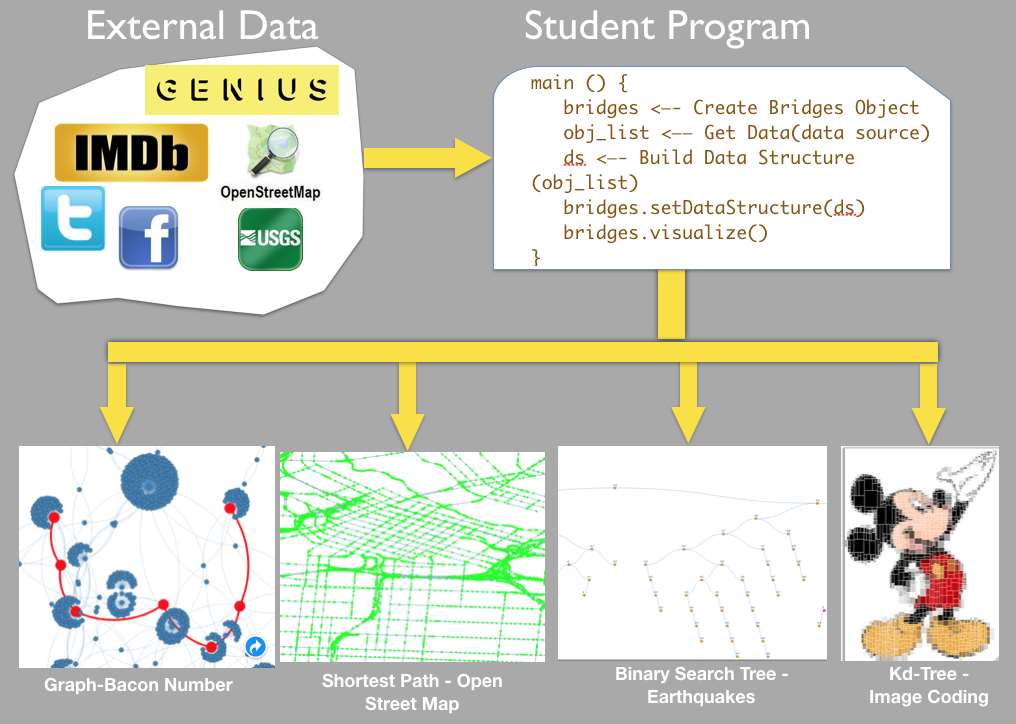
\includegraphics[width=.7\linewidth]{fig/bridges-overview.png}
\end{frame}
\begin{frame}{BRIDGES: Getting Started}
\begin{block}{BRIDGES Account, Credentials}
\begin{itemize}
	\item Go to the \href{http://bridgesuncc.github.io/}{\color{purple}\textsl{[BRIDGES Home Page]}} and create an account by using the login button (you can use your email id as user name).
	\item Click on Profile button (in the upper right corner); you will see 
	your credentials, user name, email and  API Key; you will need this API 
	key for every BRIDGES program you write (for authentication, data set access). 
	{\center
  
\includegraphics[width=.6\linewidth]{fig/login.png}
  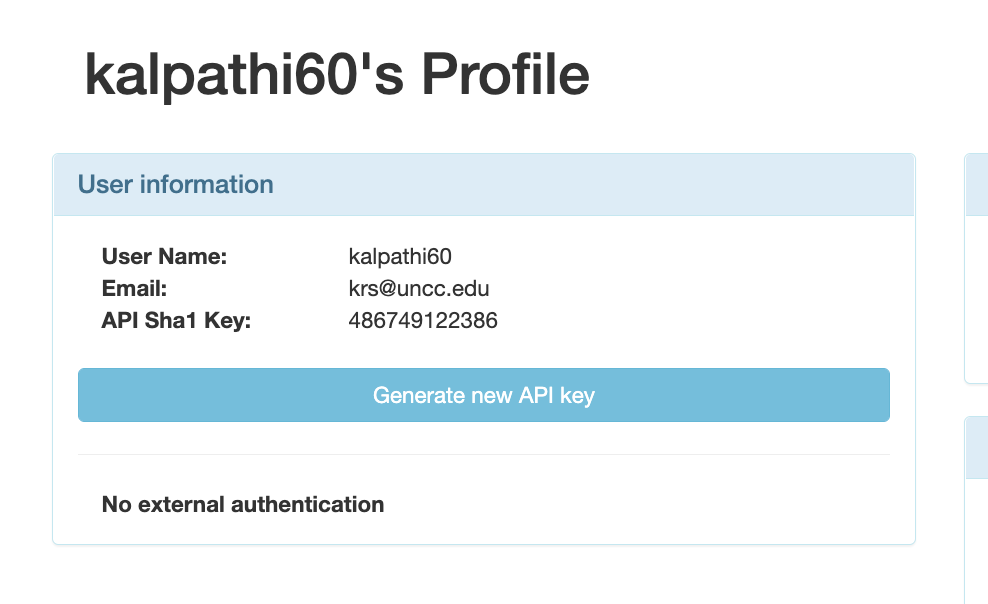
\includegraphics[width=.3\linewidth]{fig/profile.png}}

	\item Every BRIDGES program will create the Bridges object and use the 
		credentials as follows:\\
	\textsl{Bridges bridges = new Bridges(ASSIGNMENT\_NUMBER, "USER\_ID", "API\_KEY")}
\end{itemize}
\end{block}
\end{frame}
\begin{frame}{BRIDGES: Getting Started}
\begin{block}{BRIDGES Configuration/Installation}
\begin{itemize}
	\item \textbf{Java [JDK 8.0 and above]:}
	\begin{itemize}
		\item Download the BRIDGES JAR file from the Downloads link on the 
			Bridges website.
		\item Augment your Java class path to include the path to the BRIDGES JAR file.
	\end{itemize}
	\item \textbf{C++ [C++ 14 and above]:}
	\begin{itemize}
		\item Download the BRIDGES C++ archive  from the Downloads link on the 
			Bridges website.
		\item BRIDGES C++ uses the Curl library. This will need to be installed
			and BRIDGES programs need to be linked to the Curl library.
		\item BRIDGES programs must be compiled with paths to the include and
			lib folders (the bridges library is only needed for the Game API).
	\end{itemize}
	\item \textbf{Python [v. 3.8 and above:]}
	\begin{itemize}
		\item Use the following command to install the Bridges python sources:\\
		\textsl{pip install bridges}
	\end{itemize}
\end{itemize}
\end{block}
\end{frame}
\begin{frame}{BRIDGES: A Concrete Example}
\begin{block}{A BRIDGES Example Program: Linked List Using IMDB Actor Movie Data}
\scriptsize
  \cpplisting[firstline=9,lastline=28]{tutorial/ListIMDB.cpp}
\end{block}
\end{frame}
\begin{frame}{BRIDGES: A Concrete Example}
\begin{block}{A BRIDGES Example Program: Linked List Using IMDB Actor Movie Data}
\begin{columns}
\scriptsize
  \column{.45\linewidth}
  \cpplisting[firstline=29,lastline=37]{tutorial/ListIMDB.cpp}

  \column{.45\linewidth}
\center
  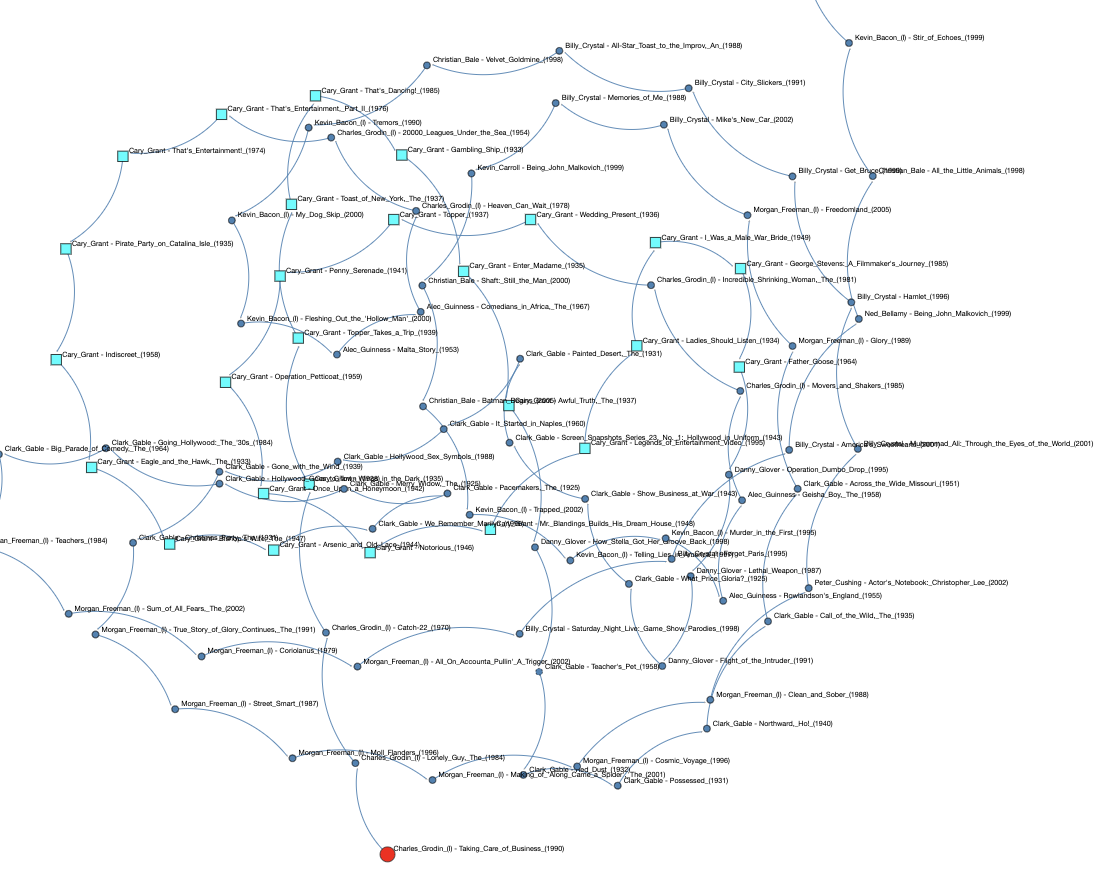
\includegraphics[width=\linewidth]{tutorial/output.png}
\end{columns}
\end{block}
\end{frame}



\end{document}
%
